\documentclass[11pt,a4paper]{article}

\usepackage[utf8]{inputenc}
\usepackage[T1]{fontenc}
\usepackage[brazil]{babel}
\usepackage{lmodern}
\usepackage{microtype}
\usepackage[a4paper,margin=2.5cm]{geometry}
\usepackage{amsmath,amssymb}
\usepackage{booktabs}
\usepackage{graphicx}
\usepackage{caption}
\usepackage{siunitx}
\usepackage[round]{natbib}
\usepackage[hidelinks]{hyperref}

\graphicspath{{../figures/}}
\sisetup{output-decimal-marker={,},group-separator={.},detect-weight=true}

\title{\textbf{A parede invisível não atravessa a fronteira:}\\
teste do efeito de número redondo de Osler (2000) para o USD/BRL}
\author{Caio Vieira\\ \small FEA.dev --- Hackathon Trainee}
\date{Julho de 2026}

\begin{document}
\maketitle

\begin{abstract}
\noindent
Números de preço ``redondos'' são amplamente tidos, na prática de mesa, como suporte e
resistência psicológicos --- uma \emph{parede invisível} que faria o preço reverter ao ser
tocada. \citet{osler2000} documentou esse efeito de forma robusta para pares de câmbio de
mercados desenvolvidos. Testamos se o mesmo mecanismo existe para o par
USD/BRL --- até onde levantamos, nunca avaliado para o Real --- replicando o desenho literal
de Osler sobre um ano de cotações intradiárias de um minuto (M1): banda de toque de
\SI{0.01}{\percent}, janela de classificação de 15 minutos, grupo de controle de 20
resistências e 20 suportes aleatórios por pregão, e teste de sinal binomial mensal.
Sobre \num{98694} barras M1 (2025-07-30 a 2026-07-01, \num{224} pregões, \num{13} meses),
não encontramos evidência do efeito: a frequência de reversão nos níveis redondos
($\approx \SI{55}{\percent}$) é estatisticamente indistinguível --- e por vezes levemente
inferior --- à de níveis arbitrários, em todas as grades testadas
(R\$1,00 / R\$0,50 / R\$0,10 / R\$0,05) e sob todas as variantes de robustez. Estendemos o
teste ao segundo mecanismo que a própria \citet{osler2000} cita como fonte dos níveis
publicados por analistas --- extremos locais (mínimos/máximos, \emph{swing points}) --- com
uma operacionalização própria (fractal de 5 dias), já que o algoritmo exato dela para esse
teste está num paper-irmão não publicado \citep{osler2000b}; o resultado é o mesmo nulo. Um
\emph{event-study} do retorno assinado pós-toque corrobora visualmente o nulo. A extensão de
aceleração pós-rompimento (H1b) só aparece em um teste agregado de Monte Carlo que
\emph{também} acende no placebo de falsificação (R\$0,01) e nos extremos locais, sendo
portanto diagnosticada como artefato de agregação, não ancoragem. Uma checagem de poder ---
injetar artificialmente um viés do tamanho do que \citet{osler2000} mediu em pares G10
($+4{,}6$ pontos percentuais) nos dados reais --- mostra que o teste o detectaria com folga,
descartando baixa potência como explicação nas grades bem povoadas. O nulo é, portanto, mais
bem explicado por diferenças reais de desenho frente a Osler: nível curado por analista vs.\
enumeração mecânica, toque bid/ask vs.\ OHLC, e microestrutura de mercado emergente vs.\ G10.
\end{abstract}

\section{Introdução}

Há uma crença difundida entre operadores de câmbio de que o preço ``respeita'' números
redondos: ao se aproximar de um nível como R\$5,00 ou R\$5,50, ele tenderia a reverter, como
se houvesse ali uma barreira. Essa intuição tem lastro empírico em mercados desenvolvidos.
\citet{osler2000}, usando o livro de ordens intradiário, mostrou que taxas de câmbio de fato
revertem com mais frequência ao tocar números redondos, e ligou o fenômeno à concentração de
ordens \emph{stop-loss} e \emph{take-profit} nesses níveis --- mecanismo depois detalhado em
\citet{osler2003}. A hipótese não é folclore: é um efeito medido e explicado.

O que não sabemos é se ele \emph{atravessa a fronteira}. Toda a evidência de Osler vem de
pares líquidos de moedas fortes (dólar, iene, libra, marco). O Real é uma moeda emergente,
com microestrutura, liquidez e composição de participantes distintas. Aplicar a crença ao
USD/BRL é, na prática, importá-la sem teste. Este trabalho faz esse teste, replicando o
desenho de \citet{osler2000} da forma mais literal que os dados disponíveis permitem, e
pré-registrando todos os parâmetros antes de observar resultados, para evitar
\emph{p-hacking}.

Formulamos duas hipóteses direcionais:
\begin{itemize}
  \item \textbf{H1a --- Reversão (\emph{bounce}).} Ao tocar um nível redondo, o preço reverte
  com mais frequência do que ao tocar um nível de controle não-redondo. Esta é a réplica
  literal de Osler.
  \item \textbf{H1b --- Aceleração.} Quando o preço rompe um nível redondo (não reverte), o
  movimento subsequente é maior do que após romper um nível de controle. Osler declara
  explicitamente não testar isso (\citeauthor{osler2000} escreve que a hipótese de que os
  preços passam a tender após o rompimento ``is not examined here''); entramos com H1b como
  extensão, ancorada na literatura de regras de rompimento e filtro
  \citep{alexander1961,brock1992,curcio1997}.
\end{itemize}

Testamos H1a e H1b contra dois candidatos independentes para a origem do nível psicológico:
\textbf{números redondos} (a réplica literal de Osler) e \textbf{extremos locais}
(mínimos/máximos, o segundo mecanismo que a própria \citet{osler2000} cita --- endnote 8 ---
como fonte dos níveis que analistas publicam; ver Seção~\ref{sec:metodo}).

\section{Dados}

\paragraph{Fonte primária.} Histórico M1 (um minuto, não agregado) do símbolo \texttt{USDBRL}
via MetaTrader~5, conta demo FBS-Demo, de 2025-07-30 até 2026-07-01. O símbolo é
\emph{onshore} e só cota durante o pregão brasileiro, de modo que a restrição de sessão já
vem embutida na fonte. Aplicamos ainda o filtro de sessão consistente $[15{:}30, 23{:}00)$ do
timestamp do servidor --- o equivalente brasileiro ao recorte 9h--16h de Nova York que Osler
usa para excluir o \emph{overnight} ilíquido --- resultando em \num{98694} barras ao longo de
\num{224} pregões distintos (\num{13} meses-calendário). O preço variou entre
R\$4,9232 e R\$5,6707 no período.

\paragraph{Sanity check da fonte (MT5 vs.\ PTAX oficial).} Para confirmar que o feed de
corretora demo é um proxy legítimo do USD/BRL à vista, casamos o \texttt{close} M1 com a PTAX
de venda de fechamento do Banco Central (API Olinda) no mesmo instante --- a PTAX é apurada
$\approx$13h de Brasília, dentro da nossa sessão --- por \emph{nearest match} com tolerância
de 5 minutos, em 223 dias (Figura~\ref{fig:sanity}). A correlação de nível é \num{0.998}: o
feed reproduz cada oscilação da taxa oficial, sem erro de escala, unidade ou inversão.
Detectamos, porém, um \emph{prêmio de nível} estável de $\approx +\SI{72}{bps}$
($\approx \SI{0.7}{\percent}$; mediana \SI{+71.8}{bps}, sem deriva secular), típico de cotação
sintética de conta demo. A consequência metodológica é que os níveis são ``redondos'' no
preço do feed, e o \emph{offset} os desloca frente aos redondos do mercado real: desprezível
para a grade grossa (R\$1,00 $\approx$ \SI{18}{\percent} de espaçamento), mas uma fração
não-trivial das grades finas. \emph{O nulo da grade R\$1,00 é, portanto, o mais confiável.}

\begin{figure}[htbp]
  \centering
  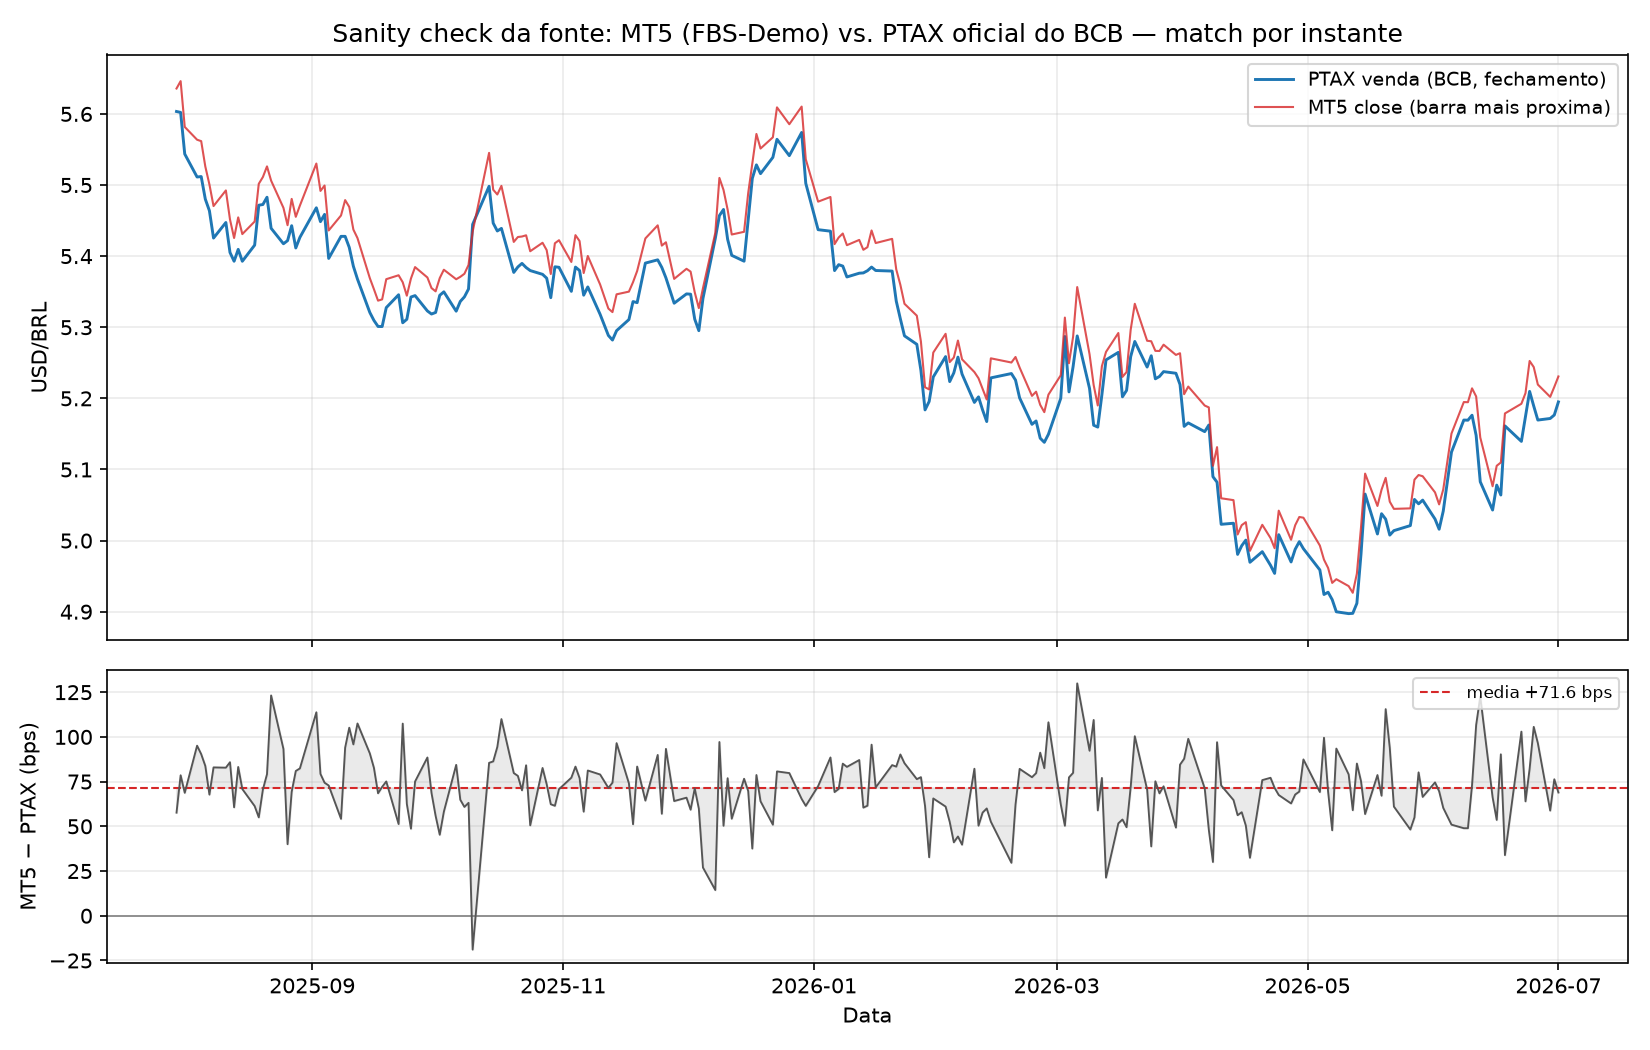
\includegraphics[width=0.85\textwidth]{sanity_ptax.png}
  \caption{Validação da fonte: \texttt{close} M1 do MT5 (FBS-Demo) contra a PTAX de
  fechamento do BCB no mesmo instante. Correlação de nível \num{0.998}; prêmio estável de
  $\approx\SI{72}{bps}$ sem deriva.}
  \label{fig:sanity}
\end{figure}

\section{Metodologia}
\label{sec:metodo}

O desenho é uma réplica direta de \citet{osler2000}, adaptada a dados M1 públicos (não
\emph{order flow} proprietário). Toda escolha foi travada antes dos resultados.

\subsection{Evento unificado}

Um único scan classifica cada toque, atendendo H1a e H1b ao mesmo tempo:
\begin{enumerate}
  \item \textbf{Banda de toque.} O preço ``toca'' um nível quando chega a \SI{0.01}{\percent}
  de distância dele (percentual, escalado pelo range observado). Robustez: \SI{0}{\percent} e
  \SI{0.02}{\percent} --- os mesmos valores de Osler.
  \item \textbf{Janela de classificação.} 15 minutos após o toque (horizonte primário de
  Osler); 30 minutos como robustez.
  \item \textbf{Classificação.} Se o preço voltou ao lado original do nível dentro da janela,
  \emph{bounce} (evidência para H1a); se permaneceu do outro lado, \emph{continuação}
  (evidência para H1b, com magnitude igual ao afastamento do nível).
\end{enumerate}

\subsection{Grupo de controle (o algoritmo de Osler)}

O controle não é \emph{offset} de grade nem \emph{bootstrap} de blocos: é o algoritmo de
níveis aleatórios do próprio Osler. Para cada pregão geram-se 20 resistências e 20 suportes
--- o número exato do paper:
\begin{align}
  R_i &= \text{Abertura}_{\text{dia}} + b_i \times \text{range}_{\text{mês}}, &
  b_i &\sim \mathcal{U}(0,1), \\
  S_i &= \text{Abertura}_{\text{dia}} - a_i \times \text{range}_{\text{mês}}, &
  a_i &\sim \mathcal{U}(0,1), \quad i = 1,\dots,20,
\end{align}
onde $\text{range}_{\text{mês}}$ é o maior \emph{gap} absoluto entre a abertura e as
máximas/mínimas intradiárias do mês. Os níveis artificiais são arredondados à precisão de
cotação (4 casas decimais para o USD/BRL). Compara-se a taxa de \emph{bounce}/continuação dos
níveis redondos reais contra a desses níveis artificiais. Usamos $N = \num{5000}$ conjuntos de
controle no run primário (Osler usa \num{10000}; a estatística de referência é uma média
sobre os conjuntos, que converge bem antes disso). A geração é feita por dia, sob demanda,
para não materializar os $\approx$45 milhões de níveis em memória.

\subsection{Granularidade dos níveis}

Hierarquia por força decrescente: \textbf{R\$1,00 / R\$0,50 / R\$0,10 / R\$0,05}, com
\textbf{R\$0,01 como placebo de falsificação} --- um nível ``redondo'' fraco demais para ter
efeito psicológico, que serve de checagem negativa: se acender, é sinal de artefato, não de
ancoragem.

\subsection{Extremos locais: segundo mecanismo candidato}
\label{sec:local}

\citet{osler2000} não deriva os níveis do teste central do paper a partir de nenhum
algoritmo --- eles são publicados por seis firmas de análise técnica, e ela apenas
\emph{observa}, a posteriori, que terminam em 0 ou 5 em \SI{96}{\percent} dos casos. A
endnote~8 do mesmo paper revela que, num paper-irmão não publicado
\citep{osler2000b}, ela testou isoladamente se números redondos \emph{ou} extremos locais
(mínimos/máximos) --- os dois insumos que as firmas mais citam para escolher níveis --- têm
poder preditivo próprio. Ela reporta que ambos têm, embora nenhum dos dois explique sozinho
todo o poder preditivo dos níveis publicados.

Esse paper-irmão não está disponível publicamente, e o algoritmo exato que Osler usou para
extremos locais não foi localizado. Implementamos, portanto, uma
\textbf{operacionalização própria e documentada} desse segundo mecanismo --- ao contrário do
controle 20R+20S (réplica literal), este não é uma réplica de um método conhecido:

\begin{itemize}
  \item \textbf{Definição (fractal clássico de \emph{swing point}).} Um dia é um máximo local
  (``resistência'') confirmado se seu \emph{high} for maior que o de \emph{todos} os $k=5$
  dias de pregão anteriores e seguintes; simétrico para mínimo local (``suporte'') via
  \emph{low}. $k=5$ é o fractal padrão de 5 barras (popularizado por Bill Williams).
  \item \textbf{Sem \emph{look-ahead}.} A confirmação só é possível $k$ dias depois do dia
  candidato; o nível só entra na lista de ``ativos'' a partir do dia seguinte à confirmação.
  \item \textbf{Roster diário.} Os 20 máximos + 20 mínimos confirmados mais recentemente até
  aquele dia --- paridade estatística deliberada com o controle 20R+20S de Osler.
\end{itemize}

Testado com o mesmo teste confirmatório e o mesmo controle usados nas grades redondas; só
muda a origem do nível de tratamento.

\subsection{Teste confirmatório}

\paragraph{Primário --- sinal binomial mensal (o teste literal de Osler).} Osler não usa
percentil de Monte Carlo. O procedimento é: (i) para cada mês, calcular a \emph{bounce
frequency} dos níveis reais, $\mathrm{BP}_{\text{mês}}$; (ii) calcular a \emph{bounce
frequency} de cada conjunto de controle e tirar a média sobre os conjuntos,
$\mathrm{BA}_{\text{mês}}$; (iii) contar em quantos dos meses vale
$\mathrm{BP}_{\text{mês}} > \mathrm{BA}_{\text{mês}}$; (iv) comparar essa contagem a uma
$\mathrm{Binomial}(N_{\text{meses}}, 0{,}5)$, tomando a cauda superior (teste unilateral, pois
a hipótese é direcional). Para H1b troca-se a \emph{bounce frequency} pela magnitude média de
continuação.

\paragraph{Complementar --- p-valor empírico de Monte Carlo.} Com apenas \num{13} meses, o
sinal binomial é pouco potente (exige $\approx$10--11 meses favoráveis para $p<0{,}05$). Como
checagem mais potente reportamos em paralelo o p-valor empírico $(r+1)/(N+1)$ de
\citet{north2002}: a estatística agregada (\emph{pooled} sobre os meses) dos níveis redondos
contra a distribuição dessa mesma estatística sobre os $N$ conjuntos de controle, com
$r = \#\{T_k \ge T_{\text{obs}}\}$ --- um teste de aleatorização no espírito da
inferência por reamostragem \citep{davison1997}. Cada grade é testada; reporta-se também a correção de
Bonferroni sobre as quatro grades reais. A grade de extremos locais (Seção~\ref{sec:local}) é
testada com o mesmo aparato, mas fora dessa família Bonferroni --- é uma hipótese
independente, não uma variante aninhada da grade redonda.

\paragraph{Nota de integridade.} Uma primeira rodada usou um \emph{proxy} não-literal
(controle de 1R+1S por dia, $N=\num{2000}$, Monte Carlo como teste primário). Após obter e ler
o PDF original do NY Fed, o desenho foi corrigido para a fidelidade literal acima; o resultado
nulo de H1a se manteve entre as duas versões, o que reforça a robustez da conclusão.

\section{Resultados}

\paragraph{Resultado central: não há evidência de nenhum dos dois mecanismos de
suporte/resistência de Osler para o USD/BRL neste conjunto de dados.} A Tabela~\ref{tab:main}
traz o desenho primário (banda \SI{0.01}{\percent}, janela 15 min), para números redondos e
para extremos locais (Seção~\ref{sec:local}).

\begin{table}[htbp]
  \centering
  \caption{Teste confirmatório primário (banda \SI{0.01}{\percent}, janela 15 min).
  $p_{\text{binom}}$ é o teste literal de sinal mensal; $p_{\text{MC}}$ é o Monte Carlo
  complementar. Nenhum $p<0{,}05$ para H1a, em nenhuma grade. Os $p_{\text{MC}}$ de H1b em
  negrito são diagnosticados como artefato (ver texto), pois o placebo e os extremos locais
  acendem junto.}
  \label{tab:main}
  \small
  \begin{tabular}{llccccc}
    \toprule
    Grade & Hipótese & Meses (BP$>$BA) & Est.\ obs. & Nula (méd.) & $p_{\text{binom}}$ & $p_{\text{MC}}$ \\
    \midrule
    R\$1,00 & H1a \emph{bounce}    & 0/2  & 0,447 & 0,550 & 1,000 & 1,000 \\
    R\$0,50 & H1a \emph{bounce}    & 3/6  & 0,546 & 0,550 & 0,656 & 0,814 \\
    R\$0,10 & H1a \emph{bounce}    & 4/12 & 0,519 & 0,550 & 0,927 & 1,000 \\
    R\$0,05 & H1a \emph{bounce}    & 8/13 & 0,551 & 0,550 & 0,291 & 0,347 \\
    \addlinespace
    R\$1,00 & H1b magnitude        & 1/2  & 0,00386 & 0,00456 & 0,750 & 1,000 \\
    R\$0,50 & H1b magnitude        & 4/6  & 0,00466 & 0,00456 & 0,344 & 0,058 \\
    R\$0,10 & H1b magnitude        & 7/12 & 0,00476 & 0,00456 & 0,387 & \textbf{0,001} \\
    R\$0,05 & H1b magnitude        & 5/13 & 0,00473 & 0,00456 & 0,867 & \textbf{0,004} \\
    \addlinespace
    \textbf{R\$0,01 (placebo)} & H1a \emph{bounce} & 6/13 & 0,546 & 0,550 & 0,709 & 0,827 \\
    \textbf{R\$0,01 (placebo)} & H1b magnitude     & 6/13 & 0,00468 & 0,00456 & 0,709 & \textbf{0,025} \\
    \addlinespace
    \textbf{Extremo local} & H1a \emph{bounce} & 6/11 & 0,542 & 0,550 & 0,500 & 0,975 \\
    \textbf{Extremo local} & H1b magnitude     & 8/11 & 0,00542 & 0,00456 & 0,113 & \textbf{0,000} \\
    \bottomrule
  \end{tabular}
\end{table}

\paragraph{H1a (reversão) --- nulo, os dois testes concordam, nas duas famílias de nível.} A
taxa de \emph{bounce} nos níveis redondos não supera a de níveis arbitrários: fica igual ou um
pouco \emph{abaixo} da média nula ($\approx 0{,}55$, valor próximo do
$\approx\SI{56}{\percent}$ que a própria Osler reporta). Nenhum $p_{\text{binom}}$ nem
$p_{\text{MC}}$ fica abaixo de \num{0.05}, em nenhuma grade redonda. Os extremos locais
reproduzem exatamente o mesmo veredito ($p_{\text{binom}}=0{,}500$, $p_{\text{MC}}=0{,}975$).

\paragraph{H1b (aceleração) --- nulo pelo teste literal; o ``sinal'' do Monte Carlo é
artefato.} O sinal binomial mensal não acusa nada ($p_{\text{binom}} \ge 0{,}11$ em toda
grade, incluindo extremos locais). O Monte Carlo \emph{pooled} marca algumas grades como
significativas (R\$0,10 $\to$ 0,001; R\$0,05 $\to$ 0,004; extremo local $\to$ 0,0002),
\emph{mas marca também o placebo R\$0,01} ($p=0{,}025$), que por construção não deveria ter
efeito. Como o placebo --- e, agora, também os extremos locais, um mecanismo de nível
completamente independente --- mostram o mesmo padrão, trata-se de artefato de agregação: os
níveis redondos (e o placebo, e os extremos locais, que ladrilham quase todo o eixo de preço)
sentam sobre o caminho do preço, enquanto os controles ficam espalhados pelo range mensal,
enviesando a comparação \emph{pooled} de magnitude. O teste de sinal mensal, que compara mês a
mês contra $\mathrm{BA}_{\text{mês}}$, não cai nesse viés --- e o placebo (e os extremos
locais) o denunciam. Não há evidência crível de aceleração.

\paragraph{Corroboração visual --- event-study.} Alinhamos cada toque em $k=0$ e acompanhamos
o retorno acumulado \emph{assinado} (em bps) de $-10$ a $+30$ minutos; o sinal segue a direção
de aproximação, de modo que no eixo $y$ positivo indica continuação e negativo indica
reversão. Se H1a fosse verdadeira, a curva dos níveis redondos ficaria abaixo da de controle
no trecho pós-toque. A Figura~\ref{fig:es} mostra o contrário: pós-toque, os retornos ficam
próximos de zero e as curvas redondas coincidem com a banda de controle de Osler --- nenhum
sinal de reversão sistemática.

\begin{figure}[htbp]
  \centering
  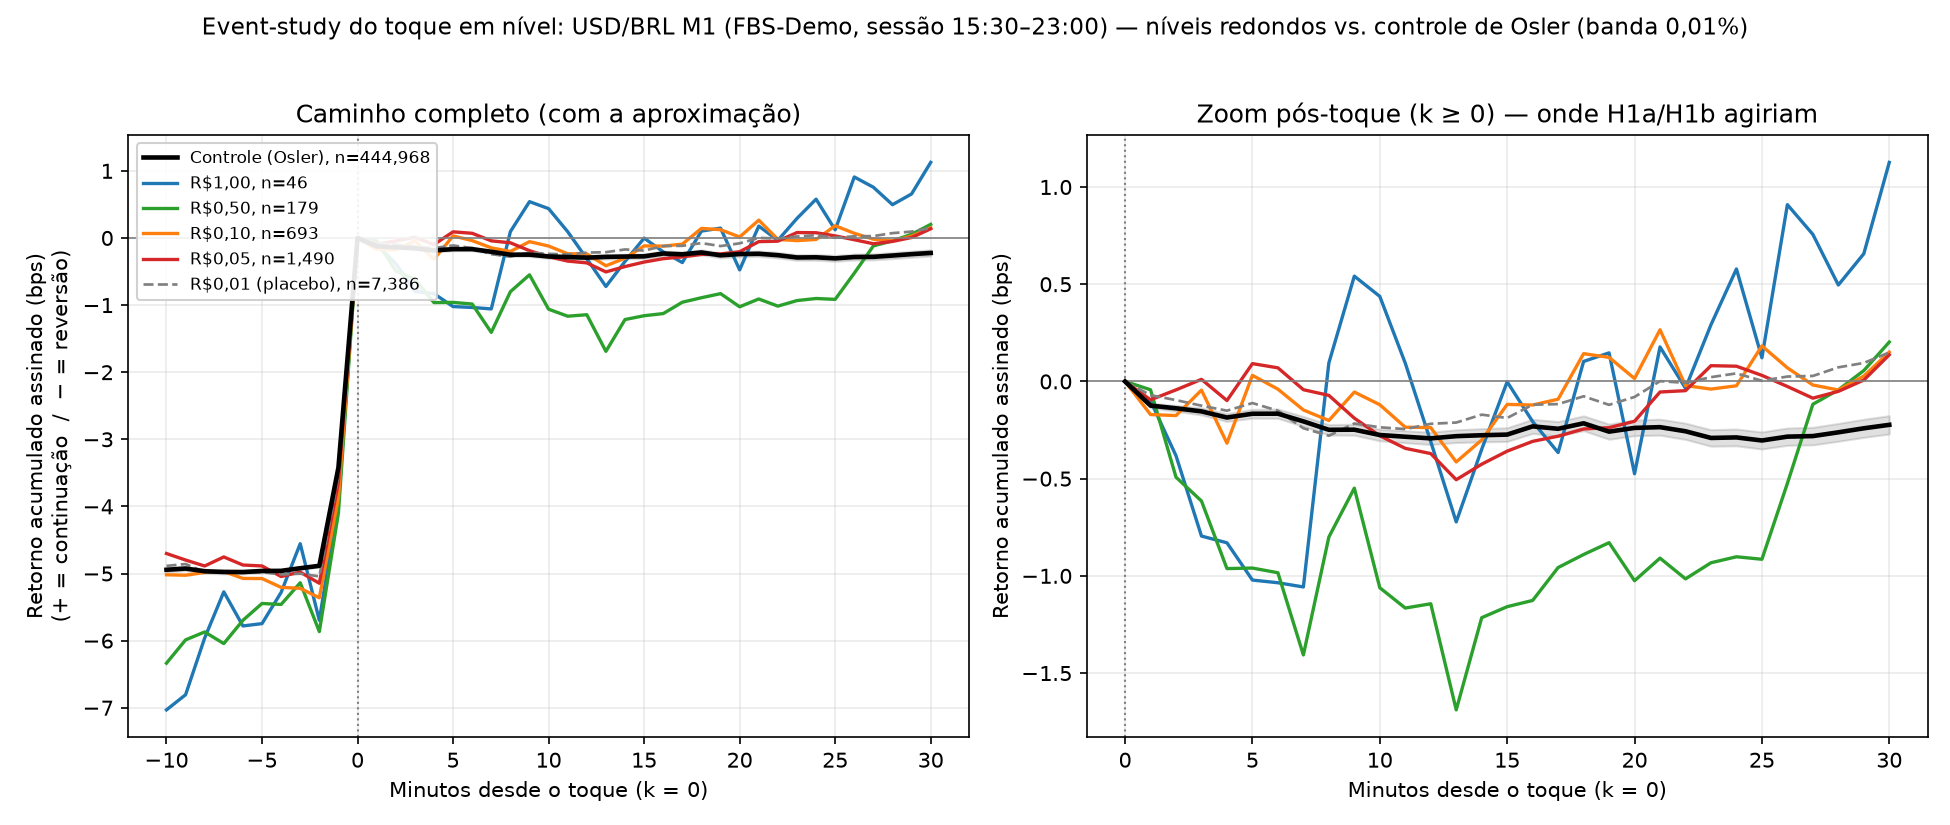
\includegraphics[width=\textwidth]{event_study.png}
  \caption{\emph{Event-study} do toque: retorno acumulado assinado (bps) contra o tempo desde
  o toque ($k=0$). Níveis redondos (R\$0,50, R\$1,00) vs.\ controle sorteado. As curvas
  redondas não se descolam da banda de controle no pós-toque. Viz com $N=25$ conjuntos de
  controle \emph{pooled}; o teste confirmatório usa $N=\num{5000}$.}
  \label{fig:es}
\end{figure}

\paragraph{Robustez.} O nulo de H1a se mantém nas variantes de banda (\SI{0}{\percent},
\SI{0.02}{\percent}) e de janela (30 min), nas duas famílias de nível. O padrão de H1b (nulo
pelo teste literal, positivo no Monte Carlo inclusive no placebo e nos extremos locais)
também se repete em todas as variantes, confirmando o diagnóstico de artefato.

\subsection{Diagnóstico do nulo}
\label{sec:diagnostico}

Diante de um nulo duplo (número redondo e extremo local), checamos diretamente se a ausência
de efeito é um artefato de implementação antes de aceitá-la como conclusão.

\paragraph{A linha de base do controle reproduz o número publicado por Osler.} A frequência de
\emph{bounce} dos níveis de controle aleatórios (a nula, sem qualquer efeito especial) ficou
em \SI{54.9}{\percent}--\SI{55.5}{\percent} neste desenho; Osler reporta \SI{56.2}{\percent}
para os níveis de controle dela (Table~8, p.~61 do paper original --- o feed de câmbio tem
autocorrelação serial negativa, de modo que \emph{qualquer} nível reverte um pouco mais da
metade das vezes, por construção). Esse número não depende de nenhuma lógica específica de
tratamento --- só do motor de detecção de toque, classificação \emph{bounce}/continuação e do
algoritmo de controle. Bater tão perto do valor publicado é evidência de que essa maquinaria
compartilhada está correta.

\paragraph{Checagem de poder: um efeito do tamanho do de Osler seria detectado?} Injetamos
artificialmente um viés de reversão controlado nos eventos \emph{reais} da grade R\$0,05
(convertendo uma fração aleatória de eventos de continuação em \emph{bounce}) e reaplicamos o
teste confirmatório real contra o controle real (Tabela~\ref{tab:power}).

\begin{table}[htbp]
  \centering
  \caption{Checagem de poder sobre a grade R\$0,05: viés de reversão injetado
  artificialmente vs.\ significância resultante no teste confirmatório real.}
  \label{tab:power}
  \small
  \begin{tabular}{ccccc}
    \toprule
    Viés injetado & \emph{Bounce} observado & $p_{\text{binom}}$ & $p_{\text{MC}}$ & Meses (BP$>$BA) \\
    \midrule
    $+0{,}0$pp (dado real) & \SI{55.1}{\percent} & 0,291 & 0,369 & 8/13 \\
    $+4{,}0$pp             & \SI{59.1}{\percent} & 0,046 & 0,002 & 10/13 \\
    $+4{,}6$pp             & \SI{59.7}{\percent} & \textbf{0,011} & \textbf{0,002} & 11/13 \\
    $+6{,}0$pp             & \SI{61.1}{\percent} & 0,011 & 0,002 & 11/13 \\
    \bottomrule
  \end{tabular}
\end{table}

$+4{,}6$ pontos percentuais não é arbitrário: é o efeito que a própria Osler mede para o marco
alemão (ela reporta $+4{,}2$pp marco, $+5{,}6$pp iene, $+4{,}0$pp libra --- p.~61). Nesse
tamanho de efeito, o teste confirmatório real acusa significância nos dois testes. Ou seja: se
o USD/BRL tivesse um efeito do tamanho do que Osler encontrou em pares G10, este pipeline o
teria detectado. O nulo observado não é, portanto, uma falha de poder estatístico nas grades
bem povoadas --- a grade R\$1,00 segue sendo um caso à parte de baixa potência (só 2 meses com
toques), discutido na próxima seção. Reproduzível com \texttt{python -m src.power\_check}.

\paragraph{Por que o efeito então não aparece? Três diferenças reais frente ao desenho de
Osler --- nenhuma delas um \emph{bug}.} \textbf{(i) Curadoria de nível, não enumeração
mecânica} --- a diferença estruturalmente mais importante. O tratamento de Osler nunca foi
``todo número redondo'': foram 2 a 18 níveis por firma por dia, escolhidos por analistas
profissionais combinando leitura de fluxo de ordens, linhas de tendência e julgamento. Este
projeto (e o próprio teste isolado de números redondos/extremos locais que Osler cita no
paper-irmão) testa, em vez disso, \emph{todo} múltiplo de R\$0,05 ou \emph{todo} ponto de
inflexão confirmado, mecanicamente. Se só uma fração dos níveis redondos/extremos é
psicologicamente relevante de fato, misturá-los com muitos níveis irrelevantes dilui qualquer
efeito real na agregação --- um problema de diluição estrutural, inerente a testar o mecanismo
diretamente, não um erro de implementação. \textbf{(ii) Definição de toque: OHLC vs.\
bid/ask.} Osler define um toque especificamente pelo lado do \emph{book} que dispararia uma
ordem real --- o \emph{bid} encostando no suporte, o \emph{ask} encostando na resistência. Os
dados brutos aqui têm uma única série OHLC, mais uma coluna de \emph{spread}
($\approx$16 pontos na amostra inspecionada) --- cerca de 3$\times$ mais larga que a própria
banda de toque de \SI{0.01}{\percent} ($\approx$5--6 pontos perto de uma cotação de 5,60). O
``toque'' medido aqui é, portanto, um proxy mais grosseiro do que dispararia de fato uma ordem
do que a definição bid/ask literal de Osler. \textbf{(iii) Estrutura de mercado: BRL vs.\
G10.} A explicação da própria Osler para o mecanismo \citep{osler2003} é a concentração de
ordens \emph{stop-loss}/\emph{take-profit} em números redondos --- característica de um
mercado G10 fortemente influenciado por mesas de análise técnica no fim dos anos 1990. O
USD/BRL é um par emergente com uma base de participantes diferente (mais fluxo macro/\emph{
carry}, menos mesa técnica de varejo); o mecanismo de concentração de ordens que sustenta o
efeito em G10 pode simplesmente ser mais fraco ou ausente aqui, independentemente de qualquer
problema de medição.

Em suma: a maquinaria de detecção/classificação reproduz a linha de base publicada por Osler e
demonstrou poder de capturar um efeito do tamanho do dela quando um é injetado. O nulo
observado é mais bem explicado por diferenças reais entre ``todo número redondo/extremo,
medido em OHLC, num par emergente'' e ``níveis curados por analistas, medidos em bid/ask, em
pares G10'' --- sendo a curadoria a diferença estruturalmente mais importante.

\section{Limitações}

\paragraph{Baixa potência --- só nas grades grossas.} Com \num{13} meses,
$\mathrm{Binomial}(13, 0{,}5)$ exige $\approx$10--11 meses com $\mathrm{BP}>\mathrm{BA}$ para
$p<0{,}05$; a grade R\$1,00 tem só 2 meses com toques, e continua sendo um nulo \emph{sob
baixa potência}. Mas a checagem de poder (Seção~\ref{sec:diagnostico}) mostra que essa
limitação \emph{não} se estende às grades bem povoadas (R\$0,05, R\$0,10, extremo local): um
efeito do tamanho do de Osler seria detectado nelas.

\paragraph{Nível curado vs.\ enumeração mecânica.} A diferença mais estrutural frente ao
desenho de Osler (Seção~\ref{sec:diagnostico}): o teste aqui usa \emph{todo} nível redondo ou
\emph{todo} extremo confirmado, não os poucos níveis que analistas profissionais efetivamente
selecionam. Isso dilui qualquer efeito real presente apenas numa fração dos níveis testados.

\paragraph{Cotação demo.} A fonte é preço de corretora demo, não \emph{order flow} real; o
prêmio de $\approx\SI{72}{bps}$ desloca os níveis redondos finos frente ao mercado. Isso
enfraquece o poder de detectar um eventual efeito nas grades finas, mas não afeta a grade
R\$1,00 (a mais confiável) nem a direção do resultado.

\paragraph{Assimetria de eventos.} Herdada do desenho de Osler, há assimetria natural entre o
número de eventos de uma grade real e de um conjunto de controle. Ainda assim, a convergência
dos dois testes para H1a e o diagnóstico de artefato para H1b tornam a conclusão robusta
dentro da amostra disponível.

\section{Conclusão}

Não encontramos evidência de que números redondos, ou extremos locais, funcionem como
suporte/resistência psicológico no USD/BRL intradiário. A frequência de reversão nesses
níveis é indistinguível da de níveis sorteados ao acaso, em todas as grades, nos dois
mecanismos candidatos e em todas as variantes de robustez; o único ``sinal'' de aceleração é
um artefato de agregação denunciado pelo próprio placebo e reproduzido de forma independente
pelos extremos locais. Isso não é, no entanto, um nulo por falta de instrumento: a linha de
base do controle reproduz a que a própria Osler publica, e uma checagem de poder mostra que um
efeito do tamanho do que ela mediu em pares G10 teria sido detectado nas grades bem povoadas
deste desenho.

A explicação mais provável para o nulo não é, portanto, ``o teste é fraco demais para ver o
efeito'' --- é que o efeito, \emph{tal como aqui operacionalizado}, provavelmente não existe
neste mercado e período, e três diferenças reais de desenho ajudam a explicar por quê: (i)
testamos \emph{todo} nível redondo ou extremo confirmado, enquanto Osler testa uma pequena
seleção curada por analistas profissionais --- diluindo qualquer efeito concentrado numa
fração dos níveis; (ii) medimos o toque em OHLC, não no bid/ask que efetivamente dispara uma
ordem, um proxy mais grosseiro do que o de Osler; e (iii) o USD/BRL é um par emergente, com
uma base de participantes provavelmente menos dominada por mesas de análise técnica de varejo
do que os pares G10 em que Osler documenta o efeito --- o mecanismo de concentração de ordens
\emph{stop}/\emph{take-profit} que ela identifica \citep{osler2003} pode ser genuinamente mais
fraco aqui. O mecanismo que \citet{osler2000} documenta de forma robusta para pares de
mercados desenvolvidos \emph{não se replica} de forma detectável para o Real neste período,
com esta operacionalização. A parede invisível, para o dólar frente ao real, parece ser menos
sobre a ausência de evidência e mais sobre uma diferença real de mercado e de desenho de
teste --- com a ressalva honesta de que níveis curados por analistas, dados de \emph{order
flow} real e uma amostra maior poderiam, em princípio, revelar um efeito que este desenho
mecânico não capta.

\paragraph{Reprodutibilidade.} Todo o pipeline (ingestão, geração de controle, testes,
extremos locais, checagem de poder, event-study, sanity check) e os snapshots de dados estão
versionados no repositório; a análise roda com \texttt{python -m src.run\_analysis}. Uma
experiência web de \emph{scrollytelling} comunica o mesmo resultado a público leigo, sem
jargão.

\bibliographystyle{plainnat}
\bibliography{refs}

\end{document}
